\documentclass[11pt,a4paper,twocolumn]{article}

\usepackage[utf8]{inputenc} 
\usepackage{graphicx}
\usepackage{physics}
\usepackage{amssymb}
\usepackage{tikz}
\usepackage{listings}
\usepackage{xcolor}
\usepackage[toc, page]{appendix}
\usetikzlibrary{quantikz}     

\usepackage[
backend=biber,
style=alphabetic,
sorting=ynt
]{biblatex}
\addbibresource{sections/references.bib}

%%%%%%%% code color %%%%%%%%%%

\definecolor{codegreen}{rgb}{0,0.6,0}
\definecolor{codegray}{rgb}{0.5,0.5,0.5}
\definecolor{codepurple}{rgb}{0.58,0,0.82}
\definecolor{backcolour}{rgb}{0.95,0.95,0.92}

\lstdefinestyle{mystyle}{
    backgroundcolor=\color{backcolour},   
    commentstyle=\color{codegreen},
    keywordstyle=\color{magenta},
    numberstyle=\tiny\color{codegray},
    stringstyle=\color{codepurple},
    basicstyle=\ttfamily\footnotesize,
    breakatwhitespace=false,         
    breaklines=true,                 
    captionpos=b,                    
    keepspaces=true,                 
    numbers=left,                    
    numbersep=5pt,                  
    showspaces=false,                
    showstringspaces=false,
    showtabs=false,                  
    tabsize=2
}

\lstset{style=mystyle}

\title{\textbf{Quantum Research Project}}
\author{Pierriccardo Olivieri}
\date{March 2020}


\begin{document}
\pagenumbering{arabic}

\twocolumn[
  \begin{@twocolumnfalse}
    \maketitle
    \begin{abstract}
        
This project aims to analyze in a computer science perspective the quantum version of random walks: the quantum walks. This model of computation can be seen as a 
building block to construct new algorithms, here we are interested in a graph application in the domain of discrete time quantum walks. The question that this research 
want to answer is if a speedup w.r.t. classical is possible and discuss eventual limitations. 



    \end{abstract}
  \end{@twocolumnfalse}
  ]

\tableofcontents

\section{Introduction}

\subsection{Acronyms}

\begin{table}[h!]
\begin{tabular}{ll}
Acronym & Extended              \\
\hline
QW      & Quantum Walk          \\
DQWL    & Discrete QW on a Line \\
DTQW    & Discrete Time QW     
\end{tabular}
\end{table}

\subsection{Random Walks}

% random walk definition
A random walk, also known as a stochastic or random process, is a mathematical object which describe a path constituted by random step over a mathematical space. A common 
example is a random walk in a line. Consider the integer set Z, starting from a certain point, for instance x = 0, the path is defined by randomly choose to move left or 
right, the movement is achieved increasing or decreasing the value of x by 1. Tossing a coin will help in choosing randomly, with equal probability, the next step to take. 
This example could be generalized by increasing the dimension of the mathematical space considered, in a cartesian plane the starting point will have two  
coordinates and the possible moves becomes 4, and there are many other possible generalizations.

%random walk discrete and continuous
Random walks can be divided in two major classes, discrete-time and continuous-time random walk. Intuitively as the names suggest the difference between this two class 
is in the time function that could be integer or real, for a more formal definition consider the random walk as a system composed by a family of random variables ${X_{t}}$
the variables $X_{t}$ will measure the system at time t, now if we consider $t\in \mathbb{N}$  is a discrete-time stochastic process, otherwise if 
$t \in \mathbb{R}^{+} \bigcup \{0\}$ is a continuous-time stochastic process. 

% final
Here we focus on the discrete-time, in particular we bind this to graphs considering the random walk on a cyclic graph of order N.

\subsection{Quantum Walks}

The Quantum version of random walks is called Quantum Walks, also here there is a distinction between the two model of discrete quantum walks and 
continuous quantum walks, the focus of this research remain in the discrete-time domain also for the quantum side. 

Following the previous example of the random walk on a line here we discuss about a discrete quantum walk on a line called coined Discrete Quantum Walk on a Line (Coined DQWL), there are also versions without coin. It's worth introducing
the Coined DQWL in a formal and generic way, then apply to a more concrete example. A formal description starts considering the three main components of a Coined DQWL: 
A walker operator, a coin, an evolution operator usually called shift operator. 

% the walker
The Walker represents the position of our system and is defined in a Hilbert space infinite but countable $\mathcal{H}_{p}$, a vector in that space represents 
the position of the walker, $\ket{position} \in \mathcal{H}_{p}$ 

% the coin
The coin operator is defined in a two-dimension Hilbert space, if we consider as basis state $\ket{0}$ and $\ket{1}$ then the coin space becomes
$\mathcal{H}_{c} = { \ket{0}, \ket{1} }$ with $\ket{coin} \in \mathcal{H}_{c}$.

The complete system finally will be in a Hilbert space composed by the Kronecker product of the two spaces above defined 

\begin{equation}
    \mathcal{H}=\mathcal{H}_{p}\otimes\mathcal{H}_{c}
\end{equation}

A state of the coined DQWL can be defined by the vector:

\begin{equation}
    \ket{\phi_{initial}} = \ket{position}_{initial} \otimes \ket{coin}_{initial}
\end{equation}

% the evolution operator
The evolution operator, also called shift operator will actually perform a step starting from the initial position, apply this operator to the
system is equal to toss a coin and depending on the outcome move the walker to the left or to the right, we can do this by increment or decrement
the actual position by 1. A possible form of the shift operator could be described by this formula:

\begin{equation}
    \scriptstyle S = \ket{0}_{c} \bra{0} \otimes \sum{i} \ket{i + 1}_{p} \bra{i} + \ket{1}_{c} \bra{1} \otimes \sum{i} \ket{i - 1}_{p} \bra{i} 
\end{equation}

Finally we can see a walker as operator itself, called U and given by:

\begin{equation}
    U = S \times (C \otimes I_{p})
\end{equation}

Applying this operator to a given system is equal to perform a step of a random walk. This explanation derives from \cite{6812670} and \cite{Kempe_2003}.
The example on the following section apply this general concept to a cyclic graph.






\section{Coined Quantum Walk}

The following example shows how to implement a Coined discrete quantum walk on a cyclic graph with N = 8 nodes. This can be achieved using the coined DQW on a line
where the line is the cylic graph. First we need to encode the graph nodes in a binary notation to fit with qubits. In general a graph with $2^{n}$ nodes needs n encoding 
bit, in our case since we have $2^{3}$ nodes we can use 3 bit to encode. The Figure 1 below shows how we can bind the qubits to the nodes of the graph.

\begin{figure}[h!]
    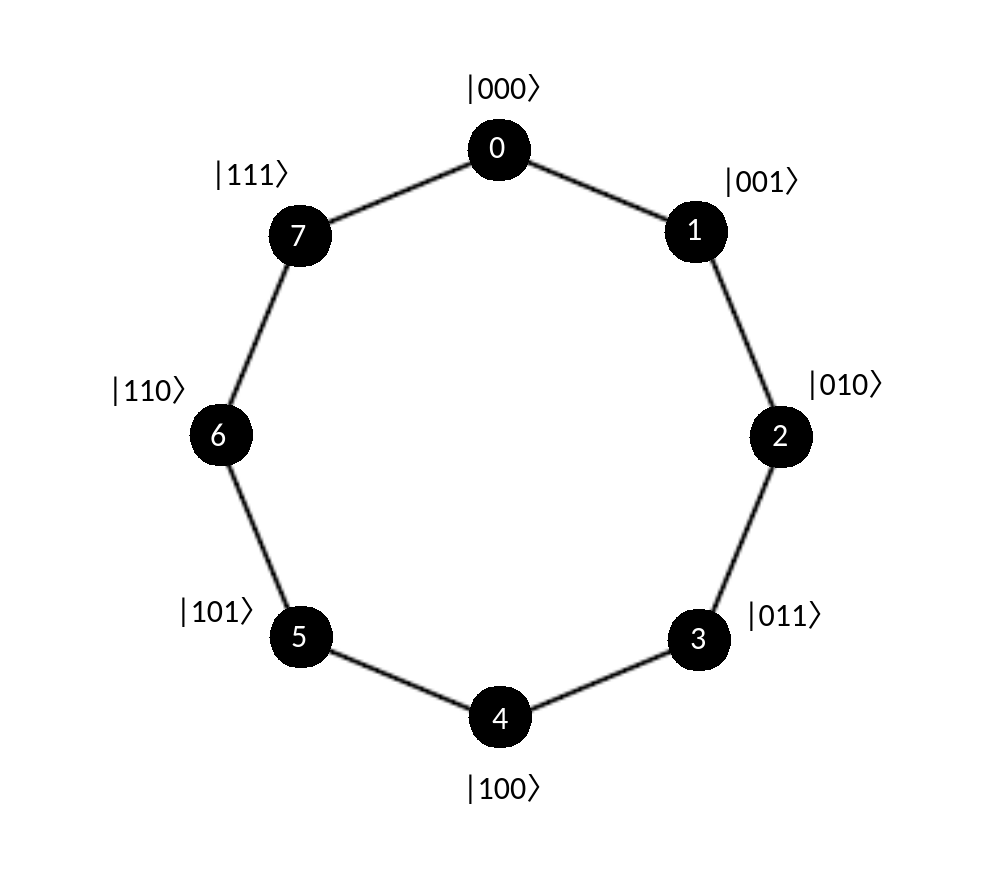
\includegraphics[scale=0.3]{img/cyclic_graph.png}
    \caption{Cyclic graph with 8 nodes, and the respective position state in qubits version}
    \centering
\end{figure}

\subsection{Components description}

We can fit now the 3 main components mentioned in the previous section for this specific example. 

% walker
Starting from the \textbf{walker operator}: for this version we need to encode the nodes of the graph in 3 qubits, usually we need log(N) qubits, in general this is not always true, 
we will see why in the next section. Using 3 qubits the postion of the walker is given by the binary encoding of the node, for instance the node 0 is represented as $\ket{000}$.

% coin operator
For the \textbf{coin operator} operator, we will use an Hadamard coin, that
consists in apply the Hadamard operator to the system. 

% hadamard coin description

% shift operator
The \textbf{shift operator} operator in this case will move the actual position that we call $\ket{i}$ to one of the adjiacent nodes, that corresponds to 
$\ket{i+1}$ or $\ket{i-1}$, which is decided by the outcome of the coin operator.

\subsection{Circuit for the CQW}

To implement the circuit in qiskit we need to translate the operator defined in quantum circuits, first we need 1 qubit for the coin and 3 for the position. 
The Hadamard can be easily implemented using an Hadamard gate on the first qubit. Then we need a circuit to perform an increment and a decrement on the initial state, 
this is less trivial and to achieve that we need two sub circuit that uses multi controlled toffoli gates. The circuit below represents an incrementer circuit 
for 3 qubits.

\begin{quantikz}
    & \ket{0} & \ctrl{2} & \ctrl{1} & \targ{}  & \qw \\
    & \ket{0} & \ctrl{1} & \targ{}  & \qw      & \qw \\
    & \ket{0} & \targ{}  & \qw      & \qw      & \qw \\
\end{quantikz}

The decrement circuit is similar but uses negative controlled not gates, the circuit below shows the decrement circuit for 3 qubits.

\begin{quantikz}
    & \ket{0} & \octrl{2} & \octrl{1} & \targ{}  & \qw \\
    & \ket{0} & \octrl{1} & \targ{}  & \qw      & \qw \\
    & \ket{0} & \targ{}  & \qw      & \qw      & \qw \\
\end{quantikz}

The negative controlled not can be represented by negate before and after the controlled not, the equivalence circuit below
clarify this explanation, for a detalied explanation look at \cite{nielsen_chuang_2010}.

$$
\begin{quantikz}[baseline={($(W.base)!.5!(W2.base) -height("$\vcenter{}$")*(0,1pt)$)}]
    & \octrl{1} & \alias{W}  \qw & \qw \\
    & \targ{}   & \alias{W2} \qw & \qw 
\end{quantikz}
=\begin{quantikz}[baseline={($(W.base)!.5!(W2.base) -height("$\vcenter{}$")*(0,1pt)$)}]
    & \gate{X}  & \ctrl{1} & \gate{X} & \qw \\
    & \qw       & \targ{}  & \qw      & \qw 
\end{quantikz}
$$

Finally the decrement circuit defined above, using this equivalence, is showed below.   

\begin{quantikz}
    & \ket{0} & \targ{} & \ctrl{2} & \ctrl{1} & \targ{} & \targ{} & \qw \\
    & \ket{0} & \targ{} & \ctrl{1} & \targ{}  & \qw     & \targ{} & \qw \\
    & \ket{0} & \targ{} & \targ{}  & \qw      & \qw     & \targ{} & \qw \\
\end{quantikz}

A similar implementation in detail is covered in \cite{douglas2007efficient}.
The final circuit by combining all the components defined is showed below.

\begin{quantikz}
    &\lstick{$\ket{0}$\\coin} & \ctrl{3} & \ctrl{2} & \ctrl{1}& \qw  & \targ{} & \ctrl{3} & \ctrl{2} & \ctrl{1} & \targ{} & \qw \\
    & \ket{0} & \ctrl{2} & \ctrl{1} & \targ{} & \qw  & \targ{} & \ctrl{2} & \ctrl{1} & \targ{}  & \targ{} & \qw \\
    & \ket{0} & \ctrl{1} & \targ{}  & \qw     & \qw  & \targ{} & \ctrl{1} & \targ{}  & \qw      & \targ{} & \qw \\
    & \ket{0} & \targ{}  & \qw      & \qw     & \qw  & \targ{} & \targ{}  & \qw      & \qw      & \targ{} & \qw \\
\end{quantikz}

It's worth to make some comments about it, this circuit represents the U operator, in fact the Hadamard coin will 
randomly choose the direction to take and activate the increment or decrement sub circuit. Therefore this corresponds
to a single iteration of the walk, by successively apply this circuit we can perform a random walk on the cyclic graph.
The code for this circuit can be found in the Appendix A at the end of this document.  


\section{Results}

The circuit obtained in the previous section can be applied to a system of 4 qubits several times to perform a random walk. 
Fig. 3 shows the results of a 100 steps random walks, obtained by applying the circuit defined in Fig.2 100 times. 

\begin{figure}[h!]
    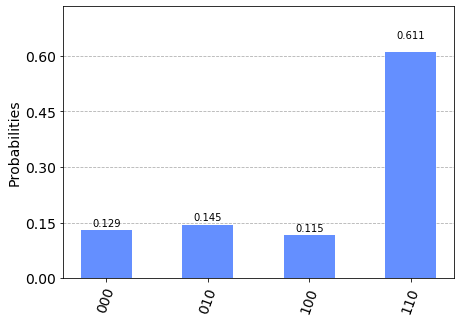
\includegraphics[scale=0.4]{img/100_steps_walk.png}
    \caption{results of a 100 step coined quantum walk}
    \centering
\end{figure}

As we can notice in Fig.4 the probailities of finding the walker in a given position are 
quite asymmetrical and also, since we started from an even number, odd numbers have zero probability of 
being measured. Differently from classical, we can 
see a true randomness behavior different from a Gaussian distribution that we will observe in a 
classical random walk. The image belowe taken from \cite{Kendon2004} shows a comparison between
the gaussian distribution of classical systems and the distribution observed for the quantum after 
100 step of the walk.

\begin{figure}[h!]
    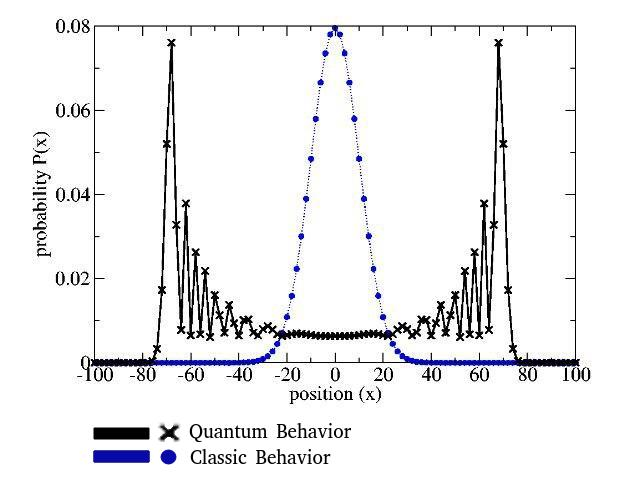
\includegraphics[scale=0.5]{img/dist.jpg}
    \caption{comparison of distribution of a 100 step random walk between classical and quantum}
    \centering
\end{figure}

This means that the walker can pass through or be in an odd(even) position but the probability to measure the Walker in a odd(even) position starting 
from an even(odd) position after 100 steps of the walk is very close to zero.  
An explanation of this behavior can be found in \cite{Kempe_2003}, this strange behavior is due to the Hadamard coin, which treats the two direction (left, right) differently. 
Considering the two states $\ket{\uparrow }$ and $\ket{\downarrow }$ this coin multiply the phase 
by -1 only in case of $\ket{\downarrow }$ inducing more cancellations of the right-wards paths.

The asymmetrical behavior can be modified by changing the initial state or 
changing the coin or balance the Hadamard coin, a more formal description of this behavior is showed in \cite{6812670}.

This particular distribution is interesting since shows that quantum can achive a true randomness, while classical computer simulate with algorithms this random behavior. 
\section{Generalizations}

The example presented is just an application to cyclic graph, also the components presented, the walker, 
the coin and the shift operator are meant to be generic. This method in fact can fit different type of problems and graph.
Starting from the coin there are many others operator that we can use, which are symmetrical, other examples are the 
balanced coins that get rid of asymmetrical behavior of the Hadamard coin. For more details
about different coins an introductory summary can be found in \cite{Kempe_2003}, but there are also Quantum walks without
the coin, as it is mentioned in \cite{6812670}.

% generalization for the graphs

The interesting thing is that the example presented can be adapted to a variety of other graphs, for instance we can
build a circuit able to perform a quantum walks also for complete graphs, hypercube, glued trees and others. 
Obviously, changing the graph, the circuit needs to be adapted but the idea remains the same. A very useful
references that shows circuits for the type of graphs mentioned is \cite{douglas2007efficient}

% multi controlled toffoli remark

An important remark concern the total qubits needed, as mentioned in the previous section if
the number of qubits is greater than 2 we need to use multi toffoli gate, this gates can be 
obtained by combining several toffoli gates, with the help of some ancillary qubits, those 
ancillary qubits are needed just to construct the multi controlled toffoli. In Fig. 5 below
is showed how to implement a multi controlled toffoli gates with 5 controls qubits, 
this image is taken from \cite{nielsen_chuang_2010}. In general following this procedure
we need a number of ancillary equals to controls qubits - 1.

\begin{figure}[h!]
    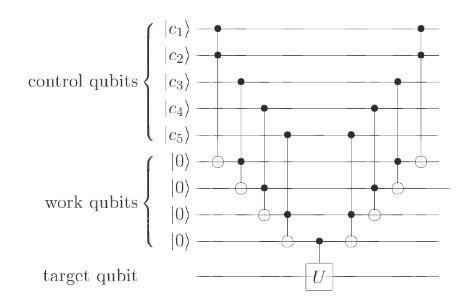
\includegraphics[scale=0.5]{img/ancillary.jpg}
    \caption{Practical representation of multi toffoli gate}
    \centering
\end{figure}

The number of ancillary qubits impacts also in the efficiency of the circuit. In the next
section will be provided a more formal description of efficiency.

\section{Performance}

To analyze the performance of quantum walks w.r.t. classical we need to define the quantum walk search problem. A more specific view of
possible applications will be discussed at the end of this document. 

% Quantum search Problem

\subsection{The search problem}

The search problem consists in find a marked vertex in a given graph by applying random walk. Given a graph G with a set of marked nodes
we want to find a marked vertex. The main idea is that starting from a vertex n we perform steps of the random walk and measure when there is an 
high probability of measure a marked vertex. 

% efficiency

\subsection{Efficiency of a QW circuit}

The implementation of a quantum walk circuit for a graph walk is said to be Efficient 
if it can be build with at most O(poly(log(N))) one and two qubits gates where N is the number of nodes in the graph \cite{douglas2007efficient}. 
An analysis of quantum walk approach w.r.t. classical is to be done for different family of graphs, since an efficient circuit
can not be realized for all the classes of graphs. The comparison between quantum and classical is made in \cite{douglas2014complexity} by 
considering the relative number of queries to a fixed oracle needed to complete the search. The paper provide two definition of 
efficiency, the first notion require the algorithm to be quadratically faster in search w.r.t. the best possible classical search and the 
second notion require the circuit to be implementable using O(log(n)) 2-qubit gates. An example of interest is the hypercube, its quantum representation can
achieve a quadratic speedup over the number of queries, said N the number of queries to an oracle we have $O(\sqrt{N})$ calls, using a coin biased 
toward marked nodes. In the paper are presented also results for complete graphs and twisted toroids.    

\subsection{Scalability and limitations of coined DTQW}

An important aspect to consider is the implementation of the controlled NOT gate. As mentioned in the previous section this gate, 
increasing the number of controls, require some ancillary qubits. In the family of graphs mentioned above in the analysis performed by 
\cite{douglas2014complexity} the number of controls qubits is O(log(N)) and the same is for the ancillary, in this case we still respect the 
notion of efficiency declared, but for sure is a parameter to consider for the scalability of these circuit. 

The method presented, as we just said, can be generalized to other types of graphs but unfortunately is limited to undirected graphs
without weights, since various application require weighted and/or directed graphs we need something more generic. In the next chapter
is showed a method that can achieve quantum walks also for undirected and weighted graphs.
\section{Szegedy quantum walk}

The following method proposed by Szegedy helps to reduce some limitations discussed in the previous section. In order to 
talk about this method we need to introduct some concepts.

\subsection{Markow chains}

A Markow chain is a stochastic process that consists in a sequence of random variables $X_{n}$ with $n \in \mathbb{Z}^{+}$
such that:

\begin{equation}
    \scriptstyle P(X_{n} | X_{n-1}, X_{n-2},...,X_{n-N}) = P(X_{n} | X_{n-1})
\end{equation}

If is time-independent can be represented by a matrix P called transition matrix. Such that the sum of each row of P is equal to 1.

\subsection{application to graphs}

We can use then a Markow Chain to represent the graph. First, considering a graph G(V,E) we construct the adjacency matrix
as follows:

\begin{equation}
    A_{i,j} = 
    \begin{cases} 
        1\, if (v_{i}, v_{j}) \in E \\
        0\, otherwise
    \end{cases}
\end{equation}

Then we can define the transition matrix P as $P_{i,j} = \frac{A_{i,j}}{indeg(j)}$ where indeg(j) 
represents the number of in-going edges of vertex j. In the 
cyclic graph $C_{8}$ (Fig. 6a) each node has 2 in-going edges therefore the transition matrix is:

\begin{equation*}
    P = \frac{1}{2}
    \begin{pmatrix}
    0 & 1 & 0 & 0 & 0 & 0 & 0 & 1 \\
    0 & 0 & 1 & 0 & 0 & 0 & 1 & 0 \\
    0 & 1 & 0 & 1 & 0 & 0 & 0 & 0 \\
    0 & 0 & 1 & 0 & 1 & 0 & 0 & 0 \\
    0 & 0 & 0 & 1 & 0 & 1 & 0 & 0 \\
    0 & 0 & 0 & 0 & 1 & 0 & 1 & 0 \\
    0 & 0 & 0 & 0 & 0 & 1 & 0 & 1 \\
    1 & 0 & 0 & 0 & 0 & 0 & 1 & 0 \\
    \end{pmatrix}
\end{equation*}

Express the graph with this transition matrix give us more flexibility, the previous 
method used directly labels encoding and was limited to undirected graphs without weights. The Szegedy algorithm works by quantizing the markow chain, here there are no problem if the graph is directed
or has weights. 

\subsection{The szegedy QW operator}
The szegedy quantum operator seems quite similar in aspect to coined quantum walk operator but there are lot of differences in the behavior. 
The space we consider now is an Hilbert space composed by 

\begin{equation}
    \mathcal{H} = \mathcal{H}_{1}^{N} \otimes \mathcal{H}_{2}^{N}
\end{equation}

where N is the number of graph's nodes and $\mathcal{H}$ has dimension $N^2$. To understand why we can anticipate that this operator works in the bipartite graph genereted copying the original node set. 
We construct 2 sets, X and Y each containing the nodes of the original graph, the bipartite graph will be 
made by connect nodes between X and Y if they are adjacent, the Fig. 6b below will hopefully clarify this concept, it shows the bipartite graph associated
to the cycli graph $C_{8}$ showed in Fig. 6a.


\begin{figure}[h!]
    \centering   
    \subfigure[Figure A]{\label{fig:a}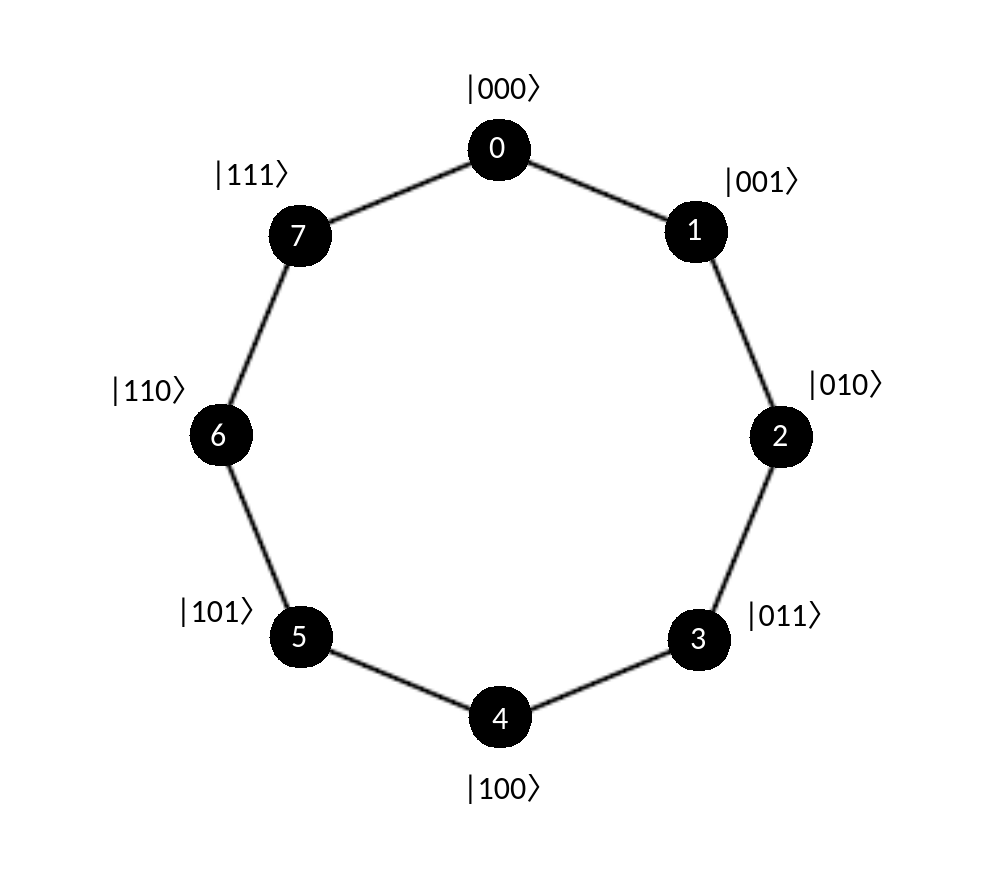
\includegraphics[scale=0.3]{img/cyclic_graph.png}}
    \subfigure[Figure B]{\label{fig:b}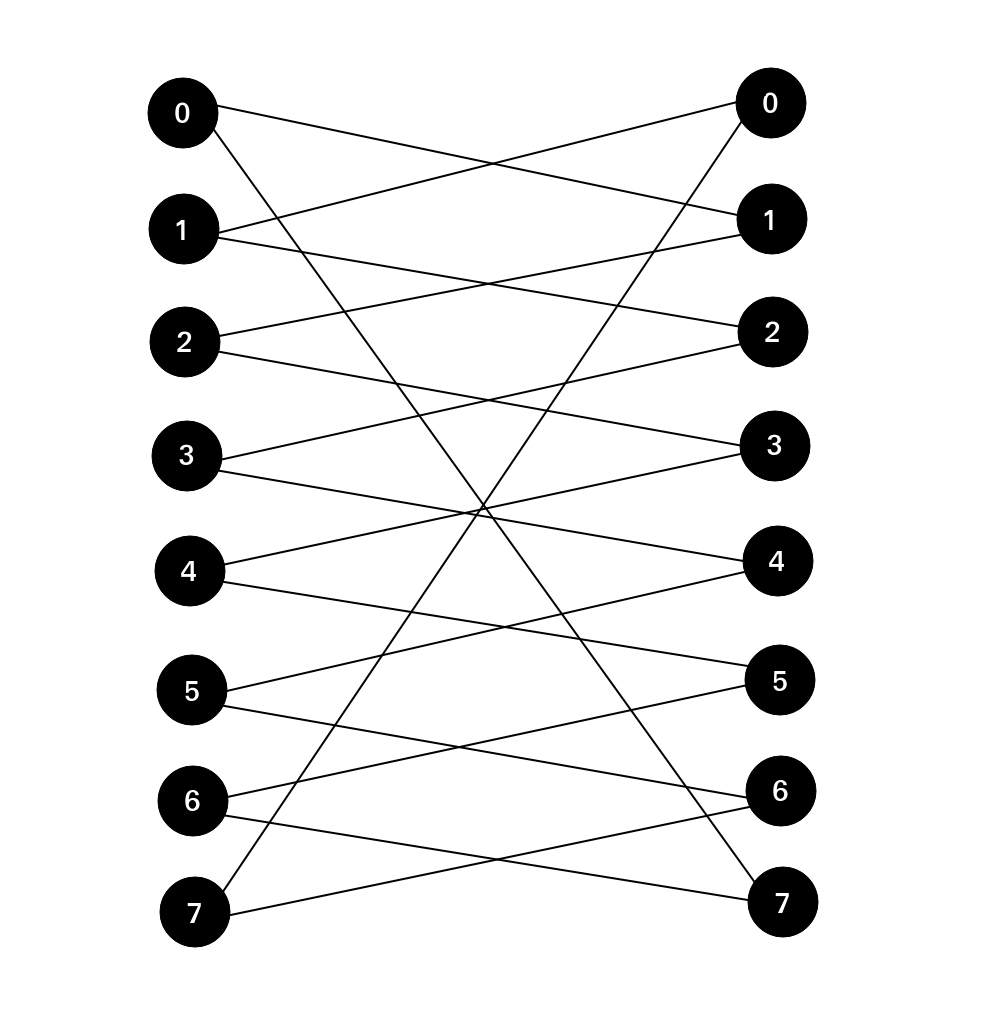
\includegraphics[scale=0.3]{img/bipartite.png}}
    \caption{Fig. A shows the cyclic graph, already used for the coined QW, Fig. B shows the correspondent bipartite graph constructed using the sets X and Y which contains the nodes of the cyclic graph
    edges connect only adjacent nodes of the cyclic graph.}
\end{figure}

Before introducing the Szegedy operator we need to define some operators that compose it, like in the coined quantum walk where the 
walk operator was composed by the coin and position operator here we have two different operators called Reflection Operator (R) and Swap Operator (S). To introduce
the R operator we need the state vector that represent the system, is given by $\ket{\psi} \in \mathcal{H}$ and is equal to:

\begin{equation}
    \ket{\psi} = \sum_{i=0}^{N-1}\sum_{j=0}^{N-1} a_{i,j}\ket{i,j} 
\end{equation}

Then we define the projector states of the markow chain:

\begin{equation}
    \ket{\psi_{i}} = \ket{i} \otimes \sum_{j=0}^{N-1}\sqrt{P_{j+1,i+1}}\ket{j} \equiv \ket{i} \otimes \ket{\phi_{i}}
\end{equation}

where $\ket{\phi_{i}}$ is the square-root of the \textit{i}-th column of the transition matrix P. The projector operator Then is given by:

\begin{equation}
    \Pi = \sum_{i=0}^{N-1}\ket{\psi{i}}\bra{\psi{i}}
\end{equation}

with the associated Reflection Operator:

\begin{equation}
    \mathcal{R} = 2\Pi - I
\end{equation}

The second operator needed is the Swap operator S given by:

\begin{equation}
    \mathcal{S} = \sum_{i=0}^{N-1}\sum_{j=0}^{N-1} \ket{i,j}\bra{j,i} 
\end{equation}

Finally the one-step Szegedy QW operator is given by:

\begin{equation}
    U_{walk} = S(I - 2\varPi) = SR
\end{equation}

This doesn't want to be a formal explanation, the schematized concepts above came from \cite{Loke_2017} and are just a summary helpful for the implementation. 
The concept behind the operator are covered with more details in \cite{c2dacf48ddf341aca084f825d3787894, Loke_2017,1366222}, 
\cite{Portugal2018} from Pag. 224 and also \cite{Wong2017} (which provides an example for a cyclic graph with 6 nodes), since \cite{c2dacf48ddf341aca084f825d3787894, Loke_2017, 1366222}
were a difficult reading for me this last two more theoretic references helped me understand some concepts and get the basic idea, especially \cite{Wong2017}. 

\section{Szegedy Quantum Walk Implementation}

For the Implementation in qiskit I used as refereces \cite{Loke_2017} and \cite{c2dacf48ddf341aca084f825d3787894}, where I also found the generic circuit 
to implement the szegedy QW on a cyclic graph.

As for the coined quantum walk, the circuit is said to be efficent if the one and two qubits gates used are no more than O(Poly(log(N))) with N number of nodes. 
While for S there are no problems R operator in this
form cannot be implemented efficiently, \cite{Loke_2017} provide a way to implement it efficiently diagonlizing the operator R. Fig. 7 taken from that
paper represent the generic circuit for the Szegedy QW on a $C_{N}$ graph and shows how R is separated in order to realize the circuit efficiently. 


\begin{figure}[h!]
    \centering   
    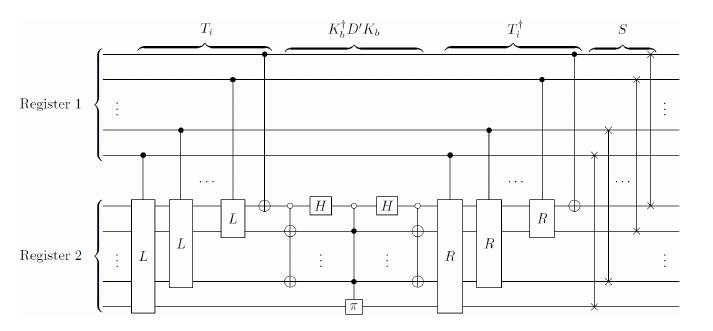
\includegraphics[scale=0.4]{img/generic_szegedy.jpg}
    \caption{Generic Circuit for the Szegedy Quantum Walk on a Cycle graph with N nodes, this image is taken from}
\end{figure}

The L and R subcircuit are called respectively one-element left rotation and one-element right rotation, are used to perform a cyclic permutation
of the vector given as input and are efficiently implementable requiring at most $log(N)$ qubits (a sequence of multi C-NOT). Swap are trivially 
efficiently implementable. In Fig. 8 below there is the specific circuit for the one-step Szegedy Quantum Walks on the cyclic graph $C_{8}$.

\begin{figure}[h!]
    \centering   
    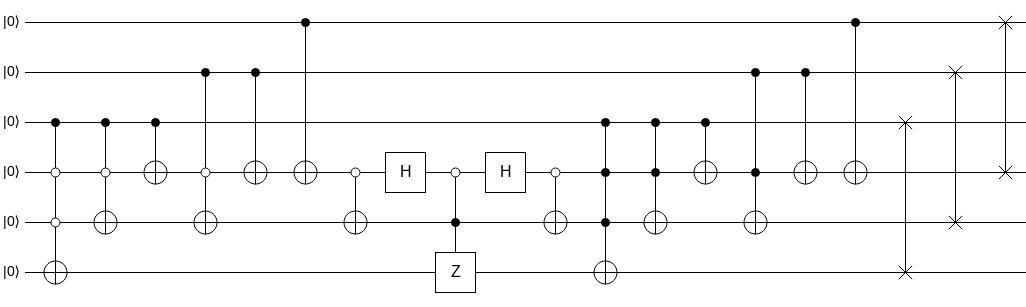
\includegraphics[scale=0.25]{img/szegedy_c8.jpg}
    \caption{Circuit for the Szegedy QW on a cyclic graph}
\end{figure}

To make an example we can prepare the initial state of the walker as a superposition $\ket{psi_{0}} = \ket{0} \otimes \ket{\phi_{0}}$
where $\ket{\phi{0}} = [0, frac{1}{\sqrt{2}}, 0 , 0, 0, 0, 0, frac{1}{\sqrt{2}}]$ and we expect as output in the first register $R_{1}$ an equiprobability of the adjacent nodes.

\href{https://algassert.com/quirk#circuit={%22cols%22:[[1,1,1,%22H%22,1,%22X%22],[1,1,1,%22%E2%80%A2%22,%22X%22],[1,1,1,%22Amps3%22],[],[1,1,1,%22Chance3%22],[1,1,%22%E2%80%A2%22,%22X%22,%22%E2%97%A6%22,%22%E2%97%A6%22],[1,1,%22%E2%80%A2%22,1,%22X%22,%22%E2%97%A6%22],[1,1,%22%E2%80%A2%22,1,1,%22X%22],[1,%22%E2%80%A2%22,1,%22X%22,%22%E2%97%A6%22],[1,%22%E2%80%A2%22,1,1,%22X%22],[%22%E2%80%A2%22,1,1,%22X%22],[1,1,1,%22%E2%97%A6%22,%22X%22],[1,1,1,%22H%22],[1,1,1,%22%E2%97%A6%22,%22%E2%80%A2%22,%22Z%22],[1,1,1,%22H%22],[1,1,1,%22%E2%97%A6%22,%22X%22],[1,1,%22%E2%80%A2%22,%22X%22,%22%E2%80%A2%22,%22%E2%80%A2%22],[1,1,%22%E2%80%A2%22,1,%22X%22,%22%E2%80%A2%22],[1,1,%22%E2%80%A2%22,1,1,%22X%22],[1,%22%E2%80%A2%22,1,%22X%22,%22%E2%80%A2%22],[1,%22%E2%80%A2%22,1,1,%22X%22],[%22%E2%80%A2%22,1,1,%22X%22],[1,1,%22Swap%22,1,1,%22Swap%22],[1,%22Swap%22,1,1,%22Swap%22],[%22Swap%22,1,1,%22Swap%22],[%22Amps3%22],[],[%22Chance3%22,1,1,%22Chance3%22]]}}{Click this simulation in Quirk} 
to see what mentioned above, again in the simulation multi controlled toffoli are specular since Quirk uses the little-endian convention.

\subsection{Comparison with classical}

The measure in which we compare those type of algorithm is in Hitting Time, this value in a stochastic process is the first time 
at which the given process "hits" a given set of substate. The famous paper of Szegedy \cite{1366222} which is the starting point of this
algorithm shows that in a certain condition we can achive a quadratic speed-up. Unfortunataly this paper was too hard for me to understand 
therfore i will not go deeper in this topic. 
\section{Applications}

The methods presented so far are meant to be general and could be applied in various context. For what I understand this is still a fresh research field 
but has a lot of potential for various applications that are difficult to solve randomized algorithm are used in context where an exact solution is too
hard to be found or too expansive computationally speaking here come these algorithms to help. For instance very famous classical problems, like 3-SAT, 
or TSP currently are solved in many case using randomized algorithm, obtaining a speed-up over the Hitting Time would be an important achievement \cite{Kempe_2003}. 
Another interesting application presented in \cite{Loke_2017} use the Szegedy Quantum Walk for the Page Rank algorithm: Quantum Page Rank algorithm. 
In \cite{Chen2019} an hybrid approach classical-quantum is used for a linear solver algorithm.


\section{Conclusions}

This research presents the analogue of random walks, the quantum walks in discrete time with a focus on graph applications. We started from 
an example of Coined quantum walk on a cycle walk to show some characteristics and difference w.r.t. classical of this method. This was just
an example, in fact this method could be generalized for other types of graphs, or for other version without coins. Then we performed
an analysis of this method applied to the problem of search a marked vertex for some family of graphs thanks to \cite{douglas2014complexity}
we know that quadratic speedup w.r.t. classical, using an efficient circuit. However the method presents some limitations, it works only for undirected and not weighted graph. The Szegedy
quantum walk helps to get rid of limitations by quantiziong the markow chain related to the graph. This method
can be efficiently implemented for the cycle graph. Some personal though about this model of computation,    
\printbibliography[title={References}]

\twocolumn[
  \begin{@twocolumnfalse}
    \appendix
    \section{Coined Quantum walk}
This code below is referred to coined quantum walk, using Hadamard coin for a
cycle graph with number of nodes N=3.
\enlargethispage{\baselineskip}

\begin{lstlisting}[breaklines,language=Python]
from qiskit import *

#increment operator for a 3-bit state register
def increment_op(circuit):
    qr = circuit.qubits
    circuit.mct([qr[0],qr[1],qr[2]],qr[3],None,mode='noancilla')
    circuit.ccx(qr[0],qr[1],qr[2])
    circuit.cx(qr[0],qr[1])
    circuit.barrier()
    return circuit

#decrement operator for a 3-bit state register
def decrement_op(circuit):
    qr = circuit.qubits
    circuit.x(qr)   
    circuit.barrier()
    circuit.mct([qr[0],qr[1],qr[2]],qr[3],None,mode='noancilla')
    circuit.ccx(qr[0],qr[1],qr[2])
    circuit.cx(qr[0],qr[1])
    circuit.barrier()
    circuit.x(qr)
    return circuit

#construct the circuit for one step of the random walk
def random_walk_step(circuit):
    #increment operator circuit
    qr_incr = QuantumRegister(4)
    increment_circ = QuantumCircuit(qr_incr, name='increment')
    increment_op(increment_circ)
    increment_inst = increment_circ.to_instruction()

    #decrement operator circuit
    qr_decr = QuantumRegister(4)
    decrement_circ = QuantumCircuit(qr_decr, name='decrement')
    decrement_op(decrement_circ)
    decrement_inst = decrement_circ.to_instruction()

    circuit.h(qr[0])
    circuit.append(increment_inst, qr[0:4])
    circuit.append(decrement_inst, qr[0:4])
    
    return circuit   

def random_walk(steps, circuit):
    for i in range(0, steps):
        random_walk_step(circuit)
    return circuit  

\end{lstlisting}
%\lstinputlisting[breaklines,breakatwhitespace,caption=inputenc,language=Python]{code/coined_quantum_walk.py}

  \end{@twocolumnfalse}
  ]
    
\end{document}